% 来源: 19c9fb8c-0672-8939-8000-0000503faebe_2.7.2_数据链路控制.pdf
% 提取时间: 2026-02-28T22:51:18+08:00

2.7.2 数据链路控制
 在数据通信领域，随着网络规模的不断扩大和数据传输速率的日益提升，数据在传输过程中面临
诸多挑战，流量控制和差错控制应运而生。一方面，由于发送方与接收方的处理能力、传输速率等
存在差异，若发送方无节制地高速发送数据，接收方可能因来不及处理而导致缓冲区溢出、数据丢
失，进而引发网络拥塞，因此需要流量控制机制来协调双方的数据传输速率，确保数据有序流动
；另一方面，物理信道存在噪声、干扰，网络设备故障、信号衰减等因素，使得数据在传输过程中
不可避免地会出现比特错误、帧丢失等问题，为了保证接收方获取到与发送方一致的准确数据，差
错控制机制至关重要，它能有效检测错误并进行纠正或重传，保障数据的完整性和可靠性。




流量控制
定义与作用
●   流量控制主要是通过限制发送方的数据发送速率，使接收方能够及时处理接收到的数据，防止
    接收方因数据接收过快而导致缓冲区溢出，进而避免数据丢失，保证数据传输的可靠性。
实现方式主要包括
● 停等协议：这是一种简单的流量控制方式。发送方发送一个数据帧后，就停止发送，等待接收
  方的确认。接收方收到数据帧后，向发送方发送确认帧。发送方只有在收到确认帧后，才会发
  送下一个数据帧。这种方式简单，但效率较低，因为发送方在等待确认时处于空闲状态，信道
  利用率不高。
● 滑动窗口协议：该协议允许发送方在未收到接收方确认的情况下，连续发送多个数据帧。发送


                                            1
     方和接收方都有一个窗口，窗口大小表示可以发送或接收的数据帧数量。发送方可以在窗口内
     发送数据帧，接收方根据自己的处理能力和缓冲区状态，调整窗口大小并反馈给发送方。发送
     方根据接收方反馈的窗口大小来控制发送速率。例如，接收方处理数据的速度较慢，就会缩小
     窗口大小，告知发送方减少发送数据的数量。滑动窗口协议提高了信道利用率，是一种较为常
     用的流量控制方式。
停止等待协议
停止等待协议很简单，在教科书中的主要意义在于建模，帮助理解协议。为此，我们先定义一些概
念和性能指标。
 ● 传输时延 Transmission time： time taken to emit all bits into medium
 ● 传播时延 Propagation time： time for a bit to traverse the link
 ● 处理时延 Processing time (delay)： time spent at the recipient or intermediate node for
   processing
 ● 排队时延 Queuing time (delay) ：waiting time at the queue to be sent out

其中传输时延和传播时延如下图所示，中文有点类似的化可以看英文，差距就远了。




停等协议链路利用率只在传输时间大于传播时间或者帧长大于链路的比特长度的情况下较高。我们来分
析一下发送一个数据块的时间

                                                                                        2
由于ack帧的传输时延较小，进一步忽略处理时延，可以简化上面的算式



链路的利用率可以表示为




定义




B=  以比特为单位的链路长度，即比特流完全占满整个链路时，链路上的比特数;
R = 链路的数据率(bps);

                                         3
d=  链路的长度，或者说距离(m);
V = 传播速率(m/s); 空气和太空中 V 是光速；对于有线，如光纤和铜 V 约为光速的0.67倍。
L = 一个帧中的比特数(以比特为单位的帧长度)
传播时间等于距离 d 除以传播速度 V ；传输时间等于用比特表示的帧长度 L 除以数据率 R 。因
此， a 实际上代表了用比特表示的媒体长度 Rd/V 与帧长度的比值。

停等协议中有一个关键细节。如果发送方发出一帧，而接收方的确认丢失或延迟了，那么发送方会重新
发送同一帧。此时，接收方可能误认为这是新的帧，从而导致重复帧的问题。为解决这一问题，停等协
议使用一个1位序列号（0或1），这样每次发送时序列号都会变化。例如，当发送方重发序列号为0的帧
时，接收方可以识别出这是之前已接收过的帧，并忽略它，同时仍然会发送确认信号以防之前的确认丢
失。




停止等待算法的主要缺点是发送方一次只能发送一个未完成的帧，这导致链路利用率低。例如，在1.5
Mbps、往返时间45 ms的链路上，延迟带宽乘积约为8 KB。由于每个往返时间（RTT）仅能发送一个1
KB的帧，因此最大发送速率仅为182 kbps，大约是链路容量的八分之一。
滑动窗口协议


                                                       4
滑动窗口协议是一种在数据链路层实现高效数据传输的技术，它允许发送方一次性连续发送多个数据帧
到接收端，而不需要等待每一个帧的确认消息（ACK）。这种机制能够显著提高数据传输效率。在该协
议中，接收端有一个固定的缓存空间大小W，用于暂时存储接收到的数据帧；相应地，发送端也维护着
一个与之相匹配的窗口大小W，在没有收到对方发来的确认信息之前，发送方最多可以连续发送W个帧。
为了确保正确无误地传输数据并避免混淆不同批次的数据帧，每个发送出去的数据帧都会被赋予一个唯
一的序号进行标识。这个序号是通过k位二进制数来表示的，因此其取值范围为0至2k-1。当达到最大值
2k-1后，序号会重新从0开始循环使用，即采用模2^k的方式进行编号。这样做不仅能够有效利用有限的
序号资源，还能保证即使是在长时间连续通信的情况下也能保持良好的同步性。
每当接收方向发送方返回一个ACK时，除了表明已经成功接收到某些特定编号的数据帧外，还会明确指
出下一个期望接收到的数据帧编号是多少。这里的RR（Recive Ready）是接收端ACK的一种形式，RRi
即表示序号为i-1的帧都收到了，可以发送第i个帧及后续帧。




         窗口大小为7(2k-1，k=3）的滑动窗口协议，请读者自己读图理解过程

接收端可以通过发送“Receive Not Ready”报文来中断对方的数据帧流。之后，为了重新激活滑动窗口
机制，接收端必须发送一个标准的确认帧。在双向通信链路中，可以采用捎带确认（piggybacking）的
方式，即在一个数据帧中同时携带待发送的数据和对之前接收数据的确认信息。如果当前没有数据需要
发送，则发送独立的确认帧。
滑动窗口协议的性能分析也相对容易。如下图所示

                                                         5
当窗口大小 W ≥ 2a + 1 时，发送端利用率 U = 1




当窗口大小 W ≤ 2a + 1 时，发送端利用率 U = 2aW+ 1   ​




差错控制
                                           6
   在数据传输过程中，为了检测错误，通常会使用循环冗余校验（CRC）等技术。这类错误检测机制能
够识别出帧在传输过程中是否发生了改变或损坏。尽管某些类型的错误检测码足够强大，甚至能够纠正
一些简单的错误，但在实际应用中，这样的纠错能力往往伴随着较高的开销，这使得它们不太适合处理
那些可能出现在网络链路上的广泛位错误或是突发性错误。特别是对于无线通信而言，由于其环境因素
更加复杂多变，即使采用了纠错编码也可能无法完全解决所有问题。因此，在面对严重损坏的数据帧
时，最直接有效的方法就是简单地将其丢弃。
   为了确保信息能够准确无误地到达目的地，需要有一种机制来可靠地从这些被丢弃（即丢失）的帧中
恢复过来。这种可靠性功能可以在链接层实现，但很多现代通信技术却忽略了这一点。实际上，可靠的
交付服务更多是在更上层——如传输层乃至应用层提供。关于究竟应该在哪一层级实现这一功能，目前
仍存在争议，这取决于多种因素，包括但不限于系统设计需求、性能考量以及成本效益分析等。我们在
此讨论可靠交付的基础概念，因为这些原则不仅适用于链接层，而且贯穿整个协议栈的不同层级，但请
注意，我们的讨论并不局限于链接层的功能。
   实现可靠交付主要依赖于两种基本机制：确认和超时。确认过程涉及发送一个小控制帧（通常称为
ACK，即Acknowledgment的缩写）回给发送方，以表明先前发送的数据帧已被成功接收。这里的“控制
帧”指的是不包含任何实际用户数据的消息头部；然而，有些协议允许将ACK信息附加到反方向流动的数
据帧之上。一旦原始发送者收到这个确认消息，就表示其之前发出的信息已经安全抵达目的地。如果发
送方在合理时间内没有接收到预期的ACK响应，则会触发一个称为“超时”的事件，并导致该帧被重新发
送。通过这种方式，可以有效地保证数据的完整性与一致性。
   利用确认和超时机制来实现可靠交付的技术通常被称为自动重传请求（ARQ, Automatic Repeat
reQuest）。接下来的部分将介绍三种不同的ARQ算法，我们将采用一种通用的语言来进行描述，而不是
深入探讨特定协议的具体实现细节。

ARQ包含三种机制
 ● Stop-and-Wait Automatic Repeat Request
 ● Go-Back-N        Automatic Repeat Request
 ● Selective Repeat Automatic Repeat Request


停等ARQ
主要针对以下两种类型的差错
 ● 帧丢失 （lost frames）
    ○ 帧没有达到另一方
 ● 帧损伤 （damaged frame）
    ○ 帧到达，但是一些比特有差错



                                                      7
源点发送一个数据帧，等待ACK
 ● 保持一个发送帧的拷贝
 ● 在终点确认返回前，源点不发送其他帧

1）帧损伤
 ● 接收端检测到差错，丢弃该帧？
 ● 发送端超时重传

2）ACK损伤
 ● 发送端超时重传
 ● 接收端收到用两份相同编号的帧
 ● 使用 ACK0 / ACK1 来确认希望接收的帧
    ○ ACKi means“I am ready to receive frame i”

执行过程如下图所示




Go-Back-N ARQ
基于滑动窗口流控机制,没有收到确认的帧的最大数目取决于窗口大小
如果没有差错，使用ACK确认接收就绪
                                                  8
 ● ACKi 表示 “I am ready to receive frame i” 或者 “I received all frames between i and my
   previous ACKs
如果错误发生，为错误帧发送rejection (negative ACK)
 ● 接收端丢弃该帧和所有后来收到的帧，直到错误帧被正确接收
 ● 发送端必须重传有差错的帧和差错帧后所有已经传输过的帧



a) 帧损伤 （Damaged frame）
 1. 接收方检测到第 i 帧中的错误
 2. 接收方发送“拒绝 i”

 3. 发送方收到“拒绝 i”

 4. 发送方重新传输第 i 帧及其后续所有帧



（1）接收端乱序
 1. 发送方发送帧 i
 2. 发送方发送帧 i+1
 3. 接收方收到失序的帧 i+1
 4. 接收方发送“拒绝 i”
 5. 发送方返回到帧 i，并重新传输它以及所有后续帧



（2）计时器超时
 1. 第i帧丢失，且没有发送额外的帧
 2. 接收方什么都没收到，既不返回确认也不返回拒绝

 3. 发送方超时，并发送一个P比特设置为1的确认帧（这实际上是一个ACK请求命令）

 4. 接收方将此解释为一个ACK请求命令，并用其期望的下一帧的编号（i）进行确认

 5. 发送方随后重新传输第i帧




                                                                                    9
Selective-Reject ARQ
选择性重传ARQ（Automatic Repeat reQuest）是一种仅针对被拒绝帧或超时帧进行重传的机制。在此
机制中，接收端会对接收到的后续帧进行缓存，从而最小化需要重传的帧数量。然而，这一方法要求接
收端具备足够大的缓存空间以支持帧的暂存。与此同时，发送端与接收端的逻辑设计更为复杂，主要体
现在以下方面：
 ● 接收端需具备按照正确顺序重组帧的能力；
 ● 发送端需能够识别并仅重传出错或失序的帧。
   这种机制特别适用于传播时延较长的卫星链路场景，在此类环境中，其高效的重传策略能够显著提
   升通信性能并降低资源浪费。




                                                         10
选择拒绝ARO对窗口大小的限制比返回N ARO更加严格。考虑这样一种情况，选择拒绝ARO序号字段的
长度为3比特，窗口大小可达到7个帧，那么设想以下情况:
1.站点A向站点B发送从帧0到帧6的所有帧。
2.站点B接收到所有的7个帧，并以RR 7作为累积确认。
3.由于噪声脉冲序列，RR 7丢失。
4.计时器超时，A重传帧0。
5.B已经将它的接收窗口向前滑动至可接受帧7,0,1,2,3,4 和5。因此它会认为丢失的是帧7，而它接收到的
是一个新的帧0，可以接受。
上述情况的问题在于发送窗口和接收窗口之间出现了重叠部分。要克服这个问题，最大窗口值必须小于
序号范围的一半。对于上述情况，只允许4个未被确认的帧存在，就不会发生混淆。一般情况，对于k比
特的序号字段，它提供的序号范围为2，而最大窗口值则限制在 2k−1 内。
性能分析
停等ARQ


                                                      11
对与停等ARQ，我们已经知道在无差错的情况下，停等协议的链路利用率是 1 +1 2a 。                     ​




如果有差错出现，则为利用率除以 Nr , Nr 是一个帧的传输次数的期望值
                                 ​       ​




         传输次数) = ∑(i × P [i次传输]) = ∑(iP (1 − P )) = 1 −1 P
                       ∞                         ∞
Nr = E(
   ​                         ​                         ​
                                                           i−1
                                                                     ​




                       i=1                       i=1

因此停等ARQ的 链路利用率是 U = 11 +− 2a
                          P
                                             ​




          ∞
用到公式 ∑(iX i−1 ) = (1 −1X)2
               ​                     ​       −1≤X ≤1
         i=1


Selective-Reject ARQ




Go-back N ARQ
                                                                         12
Each error generates a requirement to retransmit K frames rather than just
one frame.


where f(i) is the total number of frames transmitted if the original frame must be
transmitted i times




                                                                                     13
设备内流量控制
在芯片间链路上，链路错误非常罕见，恢复操作可以交给原始源计算机处理。因此，可以应用没有与错
误控制交织在一起的流量控制方法。
这张图展示了一种简单的方法，用来管理路由器内部芯片之间数据传输的流量控制。发送方有一个叫“信
用寄存器”（CR）的东西，刚开始时，它的数值等于接收方提供的缓冲区数量。发送方只有在CR的值大
于0的时候才会发送数据，并且每发送一个数据，CR的值就会减1。在接收方那边，每当它从缓冲区里处
理完一个数据，就会告诉发送方“我又有空位了”，这就是所谓的“信用”。当发送方收到这个“信用”消息
后，就会把CR的值加1，表示可以继续发送数据了。




       图片加载失败
                   基于credit的流量控制
提高性能
如果路由器分配的缓冲区数量够大—具体来说，比线路速度和往返延迟的乘积（也叫“管道大小”）还
多，那么数据就可以以全速传输。但在实际的路由器中，问题来了：通常有好几类不同的流量在共享同
一条链路。一种简单的解决办法是，把缓冲区分成几块，每类流量各自独占一部分。但这会浪费资源，
因为每类流量都需要预留出“管道大小”的缓冲区（比如10个信元缓冲区）。如果有大量类别，所需缓冲
区的数量会迅速膨胀，可能会超出路由器芯片上的静态随机存取存储器（SRAM）容量。要知道，FPGA
（现场可编程门阵列）上的SRAM本来就特别有限。

                                               14
而且，给每个类别都分配完整的管道大小其实很浪费，毕竟所有类别同时发送数据的情况很少见，即使
发生了，每个类别也只能分到链路带宽的一小部分。所以，共享缓冲区是个更合理的选择。最简单的办
法是把缓冲区分成两部分：一部分是大家共用的公共池，另一部分是每类流量专属的私有池。
一个简单的设计是，把数据信元和信用标记为属于公共池或私有池，这样可以避免不同类别互相干扰。
不过，这个方法还需要一些额外的机制，确保某个类别不会占用超过管道大小的缓冲区。
一种更优雅的方案，可以让缓冲区共享而不用标记信元。大致思路是这样的：接收方的缓冲区被分成两
部分，一部分是每类流量的私有池，包含固定数量的缓冲区（称为Min）；另一部分是一个公共池，大小
为总缓冲区减去所有私有池的总和（即B - N * Min，N是类别数量，B是总缓冲区大小）。管道大小用
Max表示。
这个协议有两种运行模式：拥塞模式和非拥塞模式。
 ● 在非拥塞模式下，每个类别最多可以占用Max个缓冲区，自由地发送数据。
 ● 在拥塞模式下，每个类别只能占用Min个缓冲区，发送受限。
    下游节点的所有缓冲区都是通用的，任何缓冲区都可以分配给任何类别的传入数据。通过精心设计
    两种模式之间的切换规则，既防止了死锁，也避免了数据丢失，同时实现了缓冲区的高效共享。
为了在不标记信元的情况下实现对私有池的管理，发送方需要跟踪两个数字：
 1. 总的未处理信元数 S ，也就是已发送的信元数减去收到的确认数。
 2. 每个类别i的未处理信元数 Si 。
    当总的未处理信元数 S 小于N * Min（即私有池还没用完时），协议处于非拥塞模式，只要某个类
                 ​




    别的未处理信元数 Si 不超过Max，它就可以继续发送数据。
    但当 S 达到或超过N * Min时，链路被认为进入了拥塞状态，此时每个类别会被限制使用私有池，
             ​




    确保 Si 不超过Min。
    简单来说，这种缓冲区共享协议的工作原理是这样的：
        ​




 ● 在轻负载时，只有少数类别在活动，这些活跃类别可以占用更多的缓冲区（最多Max个），尽可能
    快速传输数据。
 ● 在重负载时，所有类别都在活动，每个类别至少还能保证有Min个缓冲区可用，从而避免饿死。

可以添加滞后机制来防止两种模式之间的振荡。也可以将基于信用的流量控制的缓冲区共享思想扩展到
基于速率的流量控制的速率共享，例如使用漏桶算法。
提高可靠性
上一小节中概述的协议非常有效地利用了有限的接收方SRAM缓冲区，但对故障的鲁棒性不足。在了解如
何使更复杂的流量控制协议对故障具有鲁棒性之前，先从上图中描绘的更简单的信用协议入手会更明
智。
直观地说，图中的协议就像是在两家银行之间转账：“银行” 是发送方和接收方，信用和信元都算作
“钱”。很容易看出，在没有错误的情况下，系统中的总 “钱数” 是守恒的。更正式地说，设CR为信用寄
                                                  15
存器，M为从发送方到接收方传输中的信元数，c为反向传输中的信用数，Q为接收方占用的信元缓冲区
数。
那么，很容易看出（假设初始化正确，并且链路上没有信元或信用丢失），该协议在任何时刻都保持以
下属性：(CR + M + Q + C = B)，其中B是接收方的总缓冲区空间。这种关系被称为不变量，因为只要
协议正常工作，它就始终成立。建立这个不变量是协议初始化的工作，而容错机制的工作是维护这个不
变量。如果始终维护这个不变量，那么系统就永远不会丢弃信元，因为传输中的信元数加上存储的信元
数永远不会超过分配的缓冲区数量。
简单的逐跳流量控制方案存在两个潜在问题。第一，如果初始化不正确，那么发送方可能会有过多的信
用，这可能导致信元被丢弃。第二，由于链路错误，某个类别的信用或信元可能会丢失。即使是芯片间
链路也难免会偶尔出现位错误；在高链路速度下，这种错误每小时可能会发生几次。第二个问题可能会
导致速度减慢或死锁。
许多实现者可能会错误地认为这些问题可以通过简单的机制来解决。一种直接的反应是认为这些情况不
会发生或很少发生。其次，有人可能会尝试使用定时器来检测可能的死锁，以解决第二个问题。不幸的
是，很难区分死锁和接收方非常缓慢地取出信元的情况。更糟糕的是，整个链路可能会慢得像爬行一
样，导致路由器性能下降；而且结果很难调试。




                  图2标记算法的三个步骤
这些问题可能可以通过路由器重置来解决，但这是一种严厉的解决方案。相反，可以考虑以下重新同步
方案。为了清晰起见，该方案通过图2中一系列的改进来呈现。

                                                      16
在最简单的同步方案（方案1，图2）中，假设协议定期发送一个特殊标记的信元，称为标记信元。在标
记信元返回之前，发送方停止发送数据信元。在接收方，标记信元在被发送回上游节点之前先流经缓冲
区。很容易看出，在标记信元返回后，它已经 “清空” 了管道中的所有信元和信用。因此，在标记信元返
回的那一刻，协议可以将CR设置为最大值（B）。方案1很简单，但需要发送方定期空闲以进行重新同
步。
因此，方案2（图2）对方案1进行了改进，允许发送方在发送标记信元后发送信元；然而，发送方会在一
个寄存器（例如，CSM，用于记录 “自标记信元发送以来发送的信元数”）中跟踪自标记信元发送以来发
送的信元。当标记信元返回时，发送方会考虑自标记信元发送以来发送的信元，调整修正值，从而将CR
设置为(B - CSM)。
方案2的主要缺陷是无法限制标记信元在接收方队列中停留的延迟。这会导致两个问题。第一，很难确定
该方案需要多长时间才能自我纠正。第二，为了使标记信元方案本身可靠，发送方必须定期重新传输标
记信元。如果无法限制标记信元的往返延迟，发送方可能会过早重新传输，这使得在不增加序列号复杂
性的情况下，很难将标记信元的响应与请求匹配起来。
为了限制标记信元的往返延迟，方案3（图2）让标记信元绕过接收方队列并立即 “反射回来”。然而，这
要求标记信元返回时携带接收方在接收到标记信元那一刻的空闲信元缓冲区数量F。然后，当标记信元返
回时，发送方将信用寄存器CR设置为(F-CSM)。
标记信元方案是一种称为快照的经典分布式系统技术的特殊实例。非正式地说，快照是一种分布式审
计，它生成分布式系统的一致状态。我们基于标记信元的快照与Chandy和Lamport（1985）中描述的经
典快照略有不同。然而，重要的是，快照可用于检测任何分布式算法的不正确状态，并且可以在两节点
子系统中高效实现，以使任何此类协议具有鲁棒性。特别是，同样的技术（Ozveren等人，1994）可以
用于使15.1.1节中更复杂的流量控制同样具有鲁棒性。
特别是，标记信元协议使信用更新协议具有自稳定特性，即它可以从任意错误（包括链路错误）以及损
坏寄存器的硬件错误中恢复。这是一种极端形式的容错能力，可以在不牺牲性能的情况下极大地提高子
系统的可靠性。
总之，对于两节点系统的通用技术是写下协议不变量，然后设计一个定期快照来验证不变量，并在必要
时进行纠正。
内部链路条带化
路由器内部的流量控制是由互连长度不断增加和速度不断提高这两个因素驱动的。另一方面，路由器内
部的链路条带化是由互连速度较慢所驱动的。如果串行线路速度不够快，设计者可能会在内部通过多个
串行链路对信元进行条带化处理。
在大多数应用中，每个通道的延迟是可变的；在每个通道上发送数据包的最快时间和最慢时间之间存在
很大的偏差。因此，一个好的条带化算法的目标是在存在任意偏差的情况下实现先进先出（FIFO）交

                                                   17
付，路由器不应因内部机制而重新排序数据包，并且在面对链路位错误时具有鲁棒性。
为了理解为什么实现这些目标的组合可能会很困难，可以考虑循环轮询条带化。发送方以循环轮询的顺
序在通道上发送数据包。然而，如果不修改数据包，循环轮询并不能提供FIFO交付。通道可能存在不同
的延迟偏差，因此数据包在接收方的物理到达顺序可能与其逻辑顺序不同。如果没有序列号信息，数据
包可能会持续乱序。
可以通过添加数据包序列号来使循环轮询方案保证FIFO交付，接收方可以使用该序列号对数据包进行重
新排序。然而，许多实现方案不希望添加序列号，因为这会增加信元开销并降低路由器的有效吞吐量。
提高性能
为了在不增加序列号开销的前提下实现有序传输，主要思路是将物理接收和逻辑接收解耦。物理接收容
易受到延迟偏差导致的乱序影响，而逻辑接收则通过缓冲机制以及让接收方采用与发送方相同的算法来
取出信元，从而消除乱序问题。
例如，假设发送方使用一个循环指针，以循环轮询的方式在发送通道上对信元进行条带化处理。这样，
信元A会被发送到通道1，之后发送方的循环指针会递增到2。下一个信元B则会被发送到通道2，以此类
推。
接收方会缓存接收到的信元，但在信元到达时不会立即出队。相反，接收方也会维护一个初始值为通道1
的循环指针。接收方会在通道1等待接收信元，当有信元到达时，该信元会出队，然后接收方会移动到通
道2等待接收信元。因此，如果延迟偏差导致信元B（在信元A被发送到通道1之后，被发送到通道2）比
信元A先到达，接收方不会在信元A之前将信元B出队。相反，接收方会等待信元A到达，在将信元A出队
后，才会移动到通道2，并在通道2将等待的信元B出队。
提高可靠性
发送方和接收方之间的同步可能会因为单个信元的丢失而被破坏。在前面提到的循环轮询示例中，如果
在通过三条链路发送的大量信元中，信元A丢失了，接收方将会按D、B、C、G、E、F……的顺序交付数
据包，从而永久性地打乱信元顺序。




                                               18
图3 错序与恢复：接收端的最终输出为D、B、C、E、F、G、H、I，并且在逻辑上接收到E之后实现了同
步。
对于交换结构和某些链路，人们可能会认为信元丢失的情况非常罕见（比如一年一次）。然而，这样的
假设应该会让设计者感到不安，尤其是当一次丢失就可能从那时起造成永久性损害的时候。为了防止单
个信元丢失后造成永久性损害，发送方必须定期与接收方重新同步。
将一轮定义为在返回起始通道之前，对连续通道的一系列访问。在每一轮中，发送方会通过所有通道发
送数据。同样，在每一轮中，接收方会从所有通道接收数据。为了实现重新同步，发送方会维护所有通
道的轮次编号（初始值为R0），接收方也会这样做。
因此，在图3中，发送完A、B和C后，发送方所有通道的编号都变为R1。然而，在接收方，只有通道1的
编号为R1，其他通道仍为R0，这是因为在接收方的第一轮循环扫描中，第二和第三个通道还未被访问
到。当发送方或接收方的循环指针递增到某个通道时，相应的轮次编号也会递增。
实际上，轮次编号可以被视为每个通道隐含的序列号。因此，信元A可以被认为具有序列号R1，下一个在
通道1发送的信元D则可以被认为具有序列号R2，以此类推。
因此，在图3的场景2中，发送方继续在通道1发送信元D，在通道2发送信元E。接收方仍在通道1等待信
元，最终收到了信元。此时，场景切换到场景3，接收方按顺序输出信元D和B，然后移动到通道3，最终
在通道3收到信元C。
基本上，场景2中的乱序问题是由于接收方在接收方的R1轮中，将在R2轮发送的信元（即D）出队导致
的。这就提出了一种简单的同步通道轮次编号的策略：发送方应该定期在每个通道上向接收方发送其当

                                                19
前的轮次编号。为了减少开销，这样的标记信元应该在发送数百个数据信元之后再发送，代价是在信元
丢失后可能会有数百个信元出现乱序。
为简洁起见，图3中的示例假设在通道1发送信元D之后发送标记信元，其他通道上标记信元的发送情况未
展示。因此在场景3中，可以看到发送方在通道1发送了包含当前轮次编号R2的标记信元。
在场景4中，接收方按顺序输出了信元D、B和C，现在又在等待通道1上的信元。此时，包含R2的标记信
元到达。
只有当标记信元位于缓冲区头部，且循环指针指向相应通道时，接收方才会处理该标记信元。处理遵循
以下四条规则：（1）如果标记信元中的轮次编号严格大于接收方当前的轮次编号，说明标记信元到达过
早，此时循环指针递增；（2）如果轮次编号相等，那么后续的信元轮次编号会更高，因此循环指针递
增，同时标记信元被移除（但不会输出）；（3）如果标记信元中的轮次编号比当前通道的轮次编号小
1，这属于正常无错误的情况，后续的信元轮次编号将是正确的，此时标记信元被移除，但接收方的循环
指针不递增；最后，（4）如果标记信元中的轮次编号比当前通道的轮次编号小k（k>1），则表明发生了
严重错误（除信元丢失外），发送方和接收方应该重新初始化。
因此，在场景4中，规则2适用：标记信元被销毁，循环指针递增。此时，可以很容易看出，发送方和接
收方现在已完全同步，因为对于接收方的每个通道，到达该通道时的轮次编号与下一个信元的轮次编号
相等。因此，该过程在场景4中正确地将信元E出队，在场景5中将信元F出队，最后在场景6中将信元G出
队，顺序得以恢复。
因此，增强后的负载均衡算法能够快速从错误中恢复（从发送标记信元到接收标记信元的时间加上单向
传播延迟）。图3所示方法的基本技术是通过定期单向发送标记信元，检测每个通道上的状态不一致。

对于负载均衡，除了每个通道上用于关联发送方和接收方轮次编号的单向不变量之外，还有一个全局不
变量，该不变量确保在假设没有数据包丢失的情况下，通道轮次编号之间的差异不会超过1。在因数据包
丢失导致违反该不变量后，接收方会通过跳过某些信元来强制执行该节点不变量。
即使在可以给信元添加序列号的情况下，逻辑接收也有助于简化重新排序的实现过程。一些重新排序器
使用快速并行硬件排序电路来重新组装数据包。如果采用逻辑接收，这种电路就有些多余了。逻辑接收
在正常情况下已经足够，在极少数出现错误的情况下，通过缓慢扫描查找匹配的序列号就足够了。要知
道，在芯片间链路上，错误应该是非常罕见的。需要注意的是，如果添加了序列号，就能保证FIFO交
付，这与图3中的协议不同。
分布式内存
数据包缓冲区是路由器硬件的重要组成部分，原因有三：规模、普遍性和服务质量。
第一，随着速度的提升，数据包缓冲区的规模也在不断增大。经典的经验法则是，交换机应缓存RTT×R
比特的数据以应对拥塞（其中RTT是通过路由器的TCP流的平均往返时间。假设从海岸到海岸的延迟约
                                              20
为250毫秒，一个100 Gb/s的接口需要25 Gb的内存，这在商用动态随机存取存储器（DRAM）的容量范
围内，但比高速静态随机存取存储器（SRAM）大得多。
第二，数据包缓冲区在路由器中无处不在。两个重要的例子是在输入缓冲交换机的虚拟输出队列
（VOQ）输入端（由于对输出端口的竞争），以及在输出端口（由于输出链路拥塞）。然而，在实际的
路由器中，还有许多其他使用缓冲区的地方，包括上一节提到的数据包在交换结构中进行条带化处理时
的重新排序缓冲区，以及组播复制缓冲区。
第三，正如我们之前所见，服务质量（QoS）使路由器缓冲变得复杂。服务提供商使用的路由器，如思
科GSR 12000路由器，每个线路卡大约维护2000个队列，而边缘路由器，如瞻博网络的E系列，则提供
多达64000个队列，以实现精细的QoS控制。
如今，路由器缓冲区的主要问题在于，一旦链路速度超过10 Gb/s，一个最小尺寸为40字节的数据包会
在32纳秒内到达。这意味着每隔16纳秒就需要对内存进行一次数据包的写入或读取操作（请记住，数据
包必须先写入并存储，然后读取出来才能发送出去）。如果使用一个访问时间为50纳秒的标准DRAM，
这是无法实现的。同样，使用具有这种容量的SRAM成本太高且功耗太大。
一种可能的方法是设计具有更短访问时间的新型DRAM。DRAM的访问时间取决于其架构。从理论上讲，
可以通过在内部设计更小的存储体来提高DRAM的速度，甚至可以制造出访问时间为（例如）20纳秒的
DRAM。不幸的是，随着速度的提升，这种方法并不具有扩展性。此外，额外的存储体开销需要更大的
芯片面积，导致面积与成本之间的权衡难以接受。尤其在当今世界，路由器内存只是整个DRAM市场的
一小部分，而计算机内存的严格成本压力主导着DRAM市场，这种情况更为明显。
提高性能
正如上一节中，当链路成为瓶颈时我们对数据包进行跨链路条带化处理一样，许多路由器制造商通常会
在路由器内部对数据包进行跨DRAM条带化处理。这看似简单：数据包到达时，会被写入当前未被写入
的任何一个DRAM中。当一个数据包离开时，只有在其所在的DRAM空闲时，才会从该DRAM中读取数
据。需要注意的是，DRAM协议允许对同一DRAM中不同存储体的读写操作进行一定程度的流水线处理，
即使DRAM本身尚未完全完成之前对这些不同存储体的读写请求。
不幸的是，虽然这种方法在大多数情况下或系统负载较轻时可能运行良好，但在高负载和特定的访问模
式下，效果可能会很差。一些供应商试图通过增加一些加速机制来降低这种情况发生的可能性，但这种
方法仍然是基于统计的，难以准确描述。
如果需要保证最坏情况下的性能，尤其是在有严格QoS约束的情况下，这种方法是不正确的。特别是，
有几家测试公司能够发现路由器中的此类缺陷。我们需要在使用全SRAM缓冲区这种正确但昂贵的解决方
案，和跨DRAM存储体条带化这种基于统计但不正确的解决方案之间，找到一种折中的方法。
Wang等人（2010）提出了一种流水线内存系统，在以下方面具有强大的性能。该内存系统在时间t接收
到读或写请求时，能以极高的概率（例如 1 − 10−25 ）保证在 t + Δ （其中 Δ 是一个恒定延迟）时
刻准确完成请求，且适用于包括最坏情况在内的任意内存读写模式；它能够在每个SRAM周期处理一个请
                                                     21
求，因此具有与SRAM相同的吞吐量。这种统计保证是通过最坏情况大偏差理论严格证明的。该内存系统
是通用的：它不仅可以支持路由器数据包缓冲区，还可以支持其他路由器或防火墙功能，如网络流状态
的存储、访问和维护。不过，这种内存系统也有一个缺点：固定延迟 Δ 可能超过1000个SRAM周期，
即超过几微秒，对于当今的路由器和交换机来说，这个延迟有点过高。相比之下，伊耶论文中提出的内
存系统在专门用于路由器数据包缓冲区时，能提供严格的绝对（而非统计）延迟保证。它通过利用路由
器数据包缓冲区特定的内存访问模式来实现这一点。
提高可靠性
使用静态随机存取存储器（SRAM）作为动态随机存取存储器（DRAM）存储体阵列的前端缓存。通过巧
妙的算法和 “分级SRAM”，可以证明该方案能够模拟单个大型SRAM的行为。然而，要更精确地实现这
个想法，还需要做更多工作。首先，我们必须定义头部和尾部队列的大小，并证明这些大小与队列总大
小相比是较小的。其次，也是最重要的，我们必须定义算法，以确定哪些数据包从SRAM尾部缓存读入
DRAM（在输入侧），以及哪些数据包从DRAM读出到SRAM头部缓存（在输出侧）。
为了定义各种算法（具有不同的权衡）所需的头部和尾部缓存大小，我们需要以下符号。首先，很明显
DRAM与SRAM速度之比是一个基本参数。如果DRAM的访问时间是50纳秒，SRAM的访问时间是5纳
秒，那么在一次DRAM写入操作的时间内，有 10 = 50 ÷ 5 个数据包可以到达SRAM。因此，如果内存
以64字节长度的单元工作，那么缓存块（这也是从DRAM读取和写入的块大小）至少必须是640字节。
以内存单元表示的DRAM与SRAM速度之比是第一个基本参数b。
第二个基本参数是队列数量Q。显然，队列越多，SRAM和DRAM之间的潜在积压就越大。在最坏的情况
下，在等待DRAM写入时，每个队列都可能有小数据包到达。需要注意的是，每个队列只能进行一次
DRAM写入操作；不能像在同一队列中那样跨队列批量处理数据包。在写入DRAM时，通过复杂的指针管
理，理论上可以跨队列批量处理数据包。但不幸的是，在从DRAM读取数据时，这就失去了意义。从
DRAM读取的一个块现在可能包含来自不同队列、大小不一的数据，这种“分散收集”式的读取方式无法
满足动态且不可预测的读取访问模式下每个队列不同的速度需求。
尾部缓存最容易理解。直观地说，控制器会在尾部缓存中为每个队列收集最多b字节的数据，并在可能的
情况下，以一次更大的DRAM块写入操作将数据写入DRAM。因此，尾部队列大小设为 Qb 是合理的。
另一方面，头部缓存更为复杂，因为控制器必须应对来自任何队列的对抗性读取模式，而这种模式的数
量组合非常庞大。
令人惊讶的是，如果头部缓存稍微大一些（与 QblogQ 成正比），该算法就能保证在最坏情况下，无
论请求哪个队列（当然，前提是该队列有数据），头部缓存都不会出现饥饿现象。同样直观地，人们可
能会想到类似于最早截止时间优先的算法（但要证明最坏情况下 QblogQ 的界限仍需要深入思考）。
其思路是首先从DRAM中补充头部缓存中字节数最少的队列，因为对手可能接下来就会选择这个队列。
论文将此称为“最缺额队列优先”算法。由于可能存在流水线操作，实际的缺额概念更为微妙。不过，忽
略流水线操作，可以认为缺额最大的队列就是字节数最少的队列。

                                                    22
此外，如果已知队列的行为并非完全对抗性的，那么头部缓存的大小还可以进一步减小。
本节中描述的分布式内存算法产生了巨大的影响。这些算法首先在伊耶和麦基翁创立的一家名为Nemo的
初创公司中实现商业化。Nemo被思科收购后，开始对思科路由器产生重大影响。根据伊耶论文
（Sundar，2008年）中的一些估计，仅在思科内部，分布式内存每年就被用于7条以上产品线中的数百
万个芯片，通过用廉价的片外DRAM替代SRAM，每年节省数亿美元，同时支持数千个队列。虽然更复杂
的算法很少被使用，但简单的“最缺额队列优先”算法在思科绝大多数头部缓存实现中都有应用。对于尾
部缓存，大小为 Qb 的简单动态分配缓存被普遍使用。
除了节省内存，其他优点还包括降低功耗、减少专用集成电路（ASIC）上用于处理多个存储器的引脚数
量，以及提高利用率。更高的利用率来自于将数据批量处理为大小为b的块。一个令人惊讶的附带好处
是，消除了内部SRAM单元大小为64字节时发送65字节数据包所带来的棘手问题。当将一系列65字节的
数据包批量存储在大小为 b = 640 字节（例如）的尾部缓存中时，内存碎片化问题就不那么严重了。
第二个微妙的优点是，这些经过证明的在最坏情况下也能保证性能的队列消除了数据包丢失的情况：这
在存储市场以及其他对服务质量（QoS）要求严格、需要严格限制延迟的应用中至关重要。
异步更新
与快速搜索操作并发执行的原子更新，是第11章和第10章中所有增量算法的必要组成部分。例如，假设
trie树节点X指向节点Z。通常，插入一个前缀需要添加一个新节点Y，使得X指向Y，Y再指向Z。由于数
据包以线速并发到达，更新过程必须尽量减少对搜索过程的阻塞。在不使用锁的情况下，最简单的方法
是首先完全构建节点Y并使其指向Z，然后通过一次原子写入操作，将节点X的指针转向指向Y。
然而，一般来说，这样的设计存在许多需要精细处理的地方，尤其是在面临流水线等复杂情况时。为了
说明其中潜在的陷阱以及正确推理的重要性，让我们考虑下面这个取自第一个网桥实现的例子。
在第10章研究的第一个网桥产品中，网桥使用二分查找。假设有一个包含不同键B、C、D、E的长列表，
并且在最后一个（最大的）键之后有空闲空间。现在考虑添加一个新条目A的问题。有两种标准方法来处
理这个问题。
第一种方法是模仿数据库的原子更新技术，保留二分查找表的两个副本。插入A时，搜索操作在旧副本上
进行，而A被插入到第二个副本中。然后，通过一次原子操作，更新过程翻转一个指针（芯片使用该指针
来确定要搜索的表），使其指向第二个副本。
然而，这会使所需的存储空间翻倍，尤其是当内存为SRAM时，成本很高。因此，许多设计者更喜欢第二
种选择：通过将所有大于等于B的元素向下移动一个位置，为A创建一个空位。
提高性能
为了减少内存需求，更新操作必须在与搜索操作相同的二分查找表上进行。例如，在\begin{figure}[htbp]
\centering
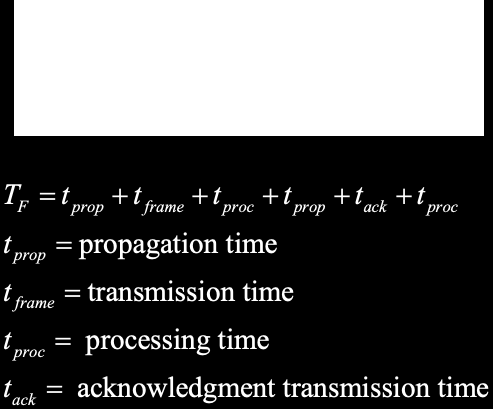
\includegraphics[width=0.8\textwidth]{../assets/ch02/ch02-2_7_2_数据链路控制-004.png}
\end{figure}
图15.4中插入元素A
时，更新操作必须将元素B、C和D向下移动一个位置。
                                                23
如果更新和搜索的设计者不同，那么对于更新设计者的常规要求通常是确保搜索过程看到的二分查找表
是一致的，且表中的键值各不相同。如果不等到完整的更新操作结束就允许进行搜索，似乎很难满足这
个要求。由于对于一个包含32000个元素的网桥数据库，一次更新可能需要很长时间，所以这种等待更
新结束再进行搜索的方式是不可接受的。
因此，可以考虑放宽要求（P3），允许二分查找表中存在重复的键值，只要该表保持有序即可。毕竟，
只要表是有序的，存在两个或更多相同值的键并不会影响二分查找的正确性。
因此，在图15.4中为A创建空位的过程是这样的：先为D创建两个条目，接着为C创建两个条目，然后为B
创建两个条目，每次操作都只对表进行一次写入。最后一步，将A写入B的第一个副本所在的位置。
为了使二分查找芯片保持简单（见第10章），路由处理器负责更新操作，而芯片负责搜索操作。表格存
储在一个单独的片外内存中；内存、处理器和芯片这三个设备可以通过一条公共总线相互通信。抽象地
说，搜索和更新这两个独立的过程同时访问内存。由于使用锁来协调内存访问会导致内存访问速度变
慢，所以这种方式并不可行。
鉴于新的规范允许存在重复键值，有人可能会试图采用最简单的内存读写原子性方式。搜索操作读取内
存，更新操作进行读写；搜索和更新的内存操作可以任意交错进行。一些实现者可能认为，因为二分查
找即使在存在重复键值的情况下也能正确工作，所以这样就足够了。
不幸的是，如图15.4所示，这种方式并不正确。在场景开始时（最左边的图），只有B、C和D分别位于
表的第一、第二和第三个条目中，第四个条目为空。对B进行搜索时从第二个条目开始；与C比较后，二
分查找算法判断应该移动到上半部分，而这里只有第一个条目。
接下来，搜索操作被延迟，同时更新操作开始通过从下往上写入重复项的方式插入A。当更新操作完成
时，B已经移动到了第二个条目。当搜索操作最后检查第一个条目时，它找到了A，并错误地得出B不在
表中的结论。
只要简单地尝试进行正确推理，就能直接发现这类反例。二分查找的标准不变量是，要么正在搜索的元
素（例如B）在当前的二分查找范围内，要么B不在表中。问题在于，更新操作可能会将正在搜索的元素
移动到当前范围之外，从而破坏这个不变量。
在网桥应用中，这种错误的唯一后果是，到达已知目的地的数据包可能会被泛洪到所有端口。这只会稍
微降低性能，不太可能被外部用户注意到！
提高可靠性
对于图15.4中的反例，一种惊慌的反应可能是放弃单副本更新，退回到更安全的双副本方式。然而，这个
反例只是表明，搜索操作必须在没有更新操作干扰的情况下完成。如果能做到这一点，二分查找的不变
量就能保持成立，结果的正确性也能得到保证。这个反例并不意味着相反的情况，即整个更新操作必须
在没有搜索操作干扰的情况下完成。相反的这种特性限制过多，会大大降低搜索速度。


                                                24
有一些简单的方法可以确保搜索操作在没有更新操作干扰的情况下完成。第一种方法是改变架构模型，
毕竟算法学就是一门通过改变问题来适应我们有限智慧的艺术。可以将所有更新写入操作集中通过搜索
芯片进行。当更新操作想要执行写入时，它向搜索芯片提交写入请求并等待确认。搜索芯片完成当前的
搜索周期后，执行所需的写入操作并发送确认信息。然后，搜索芯片可以继续处理下一个搜索任务。
第二种方法与网桥的实现方式更相符。观察发现，路由处理器负责数据包转发。路由处理器请求芯片进
行搜索，并等待几微秒获取答案。最后，路由处理器仅在没有数据包转发（因此也没有搜索操作正在进
行）时才执行更新操作。这样，更新操作可能会被搜索操作中断，但搜索操作不会被更新操作中断。
最终的解决方案依赖于搜索操作能够容忍重复键值，并且通过改变模型将更新和搜索操作集中化来避免
使用锁。需要注意的是，仅将更新操作集中化本身是不够的（如果不放宽规范以允许重复键值），因为
这将要求在没有搜索操作干扰的情况下完成整个更新操作。

不正确的分布式算法设计导致的是生产力的下降，而不是灾难性的故障。流量控制死锁可能会被路由器
重启所掩盖，信元丢失可能会被TCP重传所掩盖。内部条带化算法中未能保持数据包顺序，会导致TCP
性能下降，但不会造成数据丢失。在DRAM条带化中未能考虑所有情况，可能会导致对抗性的访问模
式，使队列出现饥饿现象和数据包丢失，不过这些数据包可以被重传。最后，不正确的二分查找表更新
只会导致数据包泛洪增加。但是，每次重启、重传、性能损失和不必要的泛洪所带来的微小损失累积起
来，可能会造成重大损失。因此，在设计路由器之间以及路由器内部的协议时要格外小心。




                                              25
